\documentclass[dvips,12pt]{article}

% Any percent sign marks a comment to the end of the line

% Every latex document starts with a documentclass declaration like this
% The option dvips allows for graphics, 12pt is the font size, and article
%   is the style

\usepackage[pdftex]{graphicx}
\usepackage{url}
\usepackage{graphicx}
\usepackage{subcaption}



% These are additional packages for "pdflatex", graphics, and to include
% hyperlinks inside a document.

\setlength{\oddsidemargin}{0.25in}
\setlength{\textwidth}{6.5in}
\setlength{\topmargin}{0in}
\setlength{\textheight}{8.5in}

% These force using more of the margins that is the default style

\begin{document}

\title{Application Server Load Testing}
\author{Sharath Rao, Yuesong Wang, Ethan Preble, Mathieu Rodrigue}
\date{\today}

\maketitle

%20151111-2115 -- m3.medium
%2151 -- m3.large
%2320 -- m3.xlarge
%

\section{Tsung Load Testing}

In this section, we describe the results from load testing with both vertically and horizontally scaled application servers.

\subsection{Vertical Scaling}

Vertical scaling was tested in 6 phases with 2, 4, 8, 16, 32, and 64 users arriving at the page every second.

\newpage

\begin{figure}[h!]
    \centering
    \begin{subfigure}[b]{0.3\textwidth}
        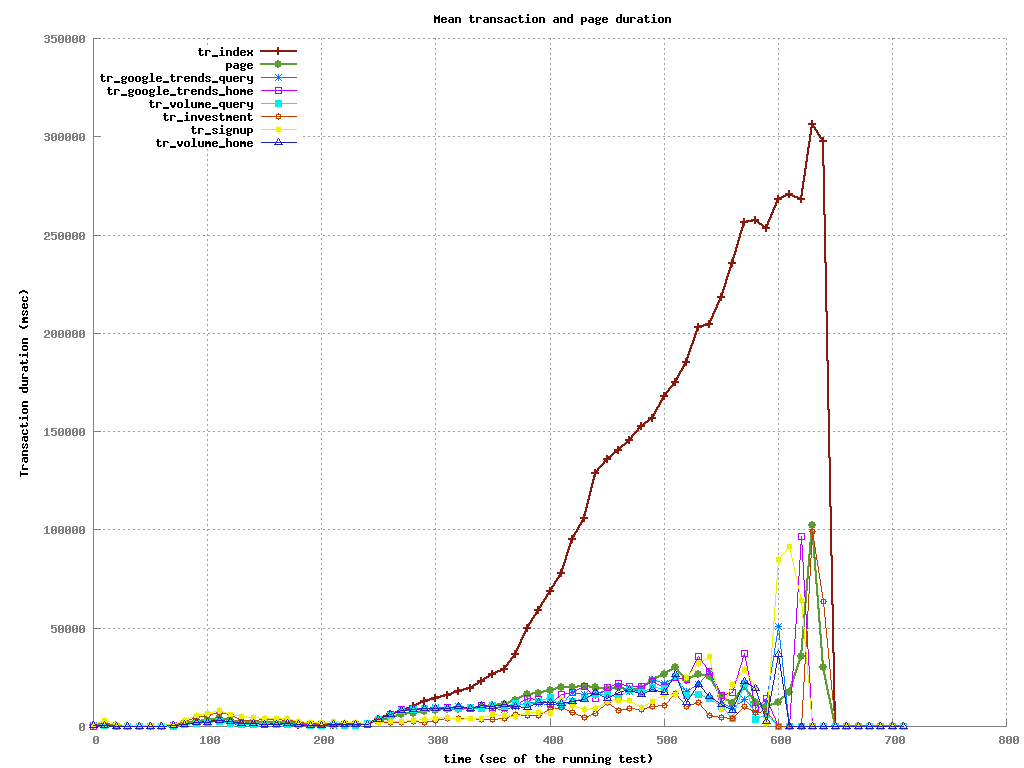
\includegraphics[width=\textwidth]{images/transaction_medium.png}
        \caption{m3.medium}
    \end{subfigure}
    ~ 
    \begin{subfigure}[b]{0.3\textwidth}
        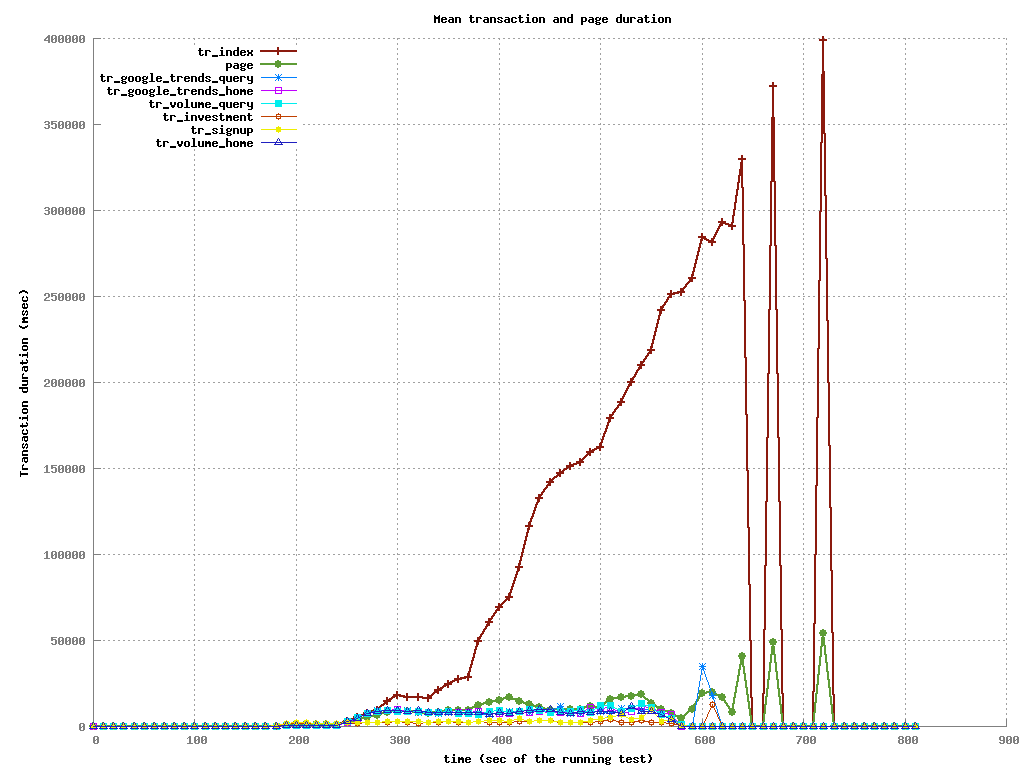
\includegraphics[width=\textwidth]{images/transaction_large.png}
        \caption{m3.large}
    \end{subfigure}
    ~ 
    \begin{subfigure}[b]{0.3\textwidth}
        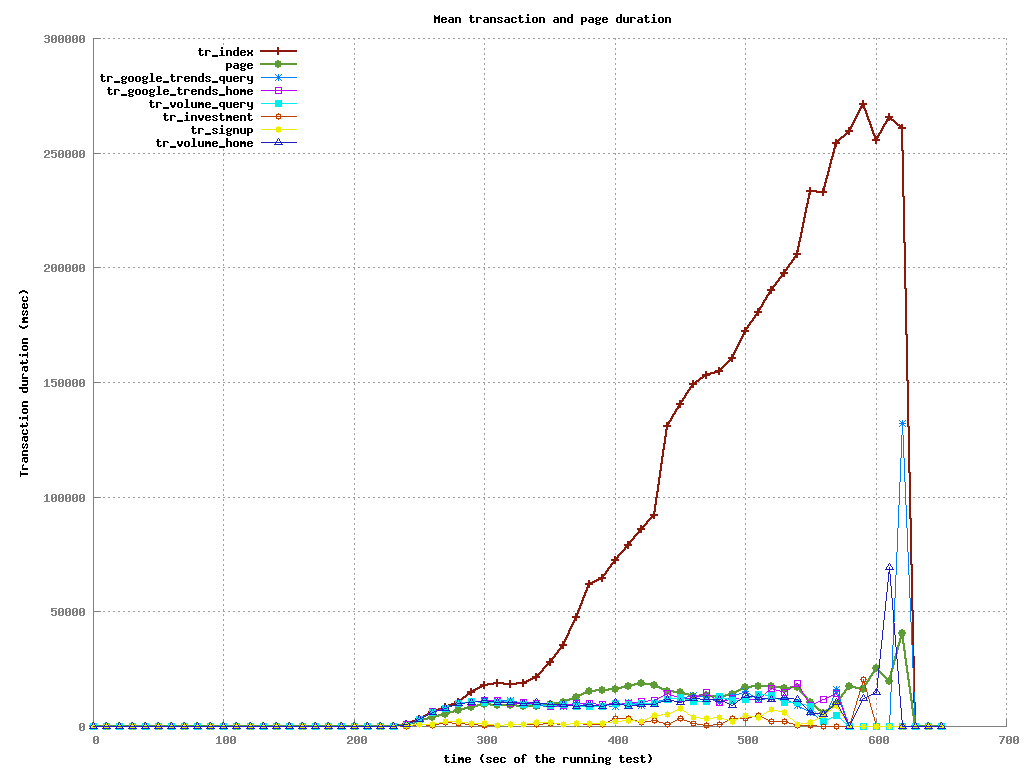
\includegraphics[width=\textwidth]{images/transaction_xlarge.png}
        \caption{m3.xlarge}
    \end{subfigure}
    \caption{Mean transaction and page duration for three m3 instances.}
\end{figure}

\begin{figure}[h!]
    \centering
    \begin{subfigure}[b]{0.3\textwidth}
        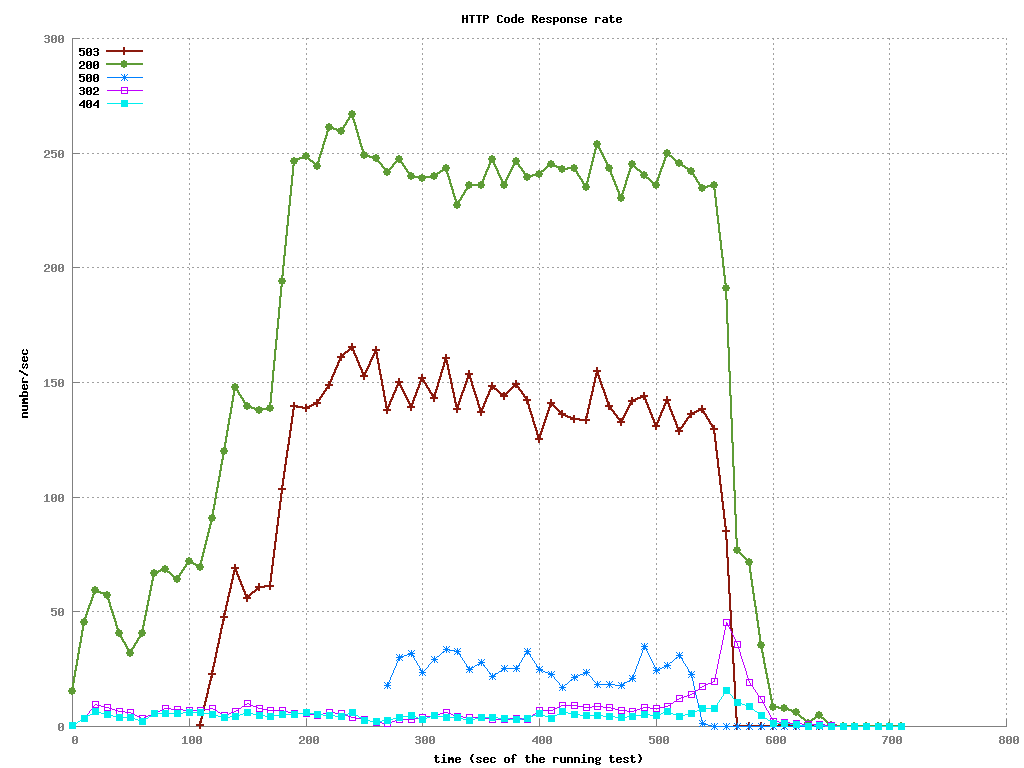
\includegraphics[width=\textwidth]{images/http_code_medium.png}
        \caption{m3.medium}
    \end{subfigure}
    ~ 
    \begin{subfigure}[b]{0.3\textwidth}
        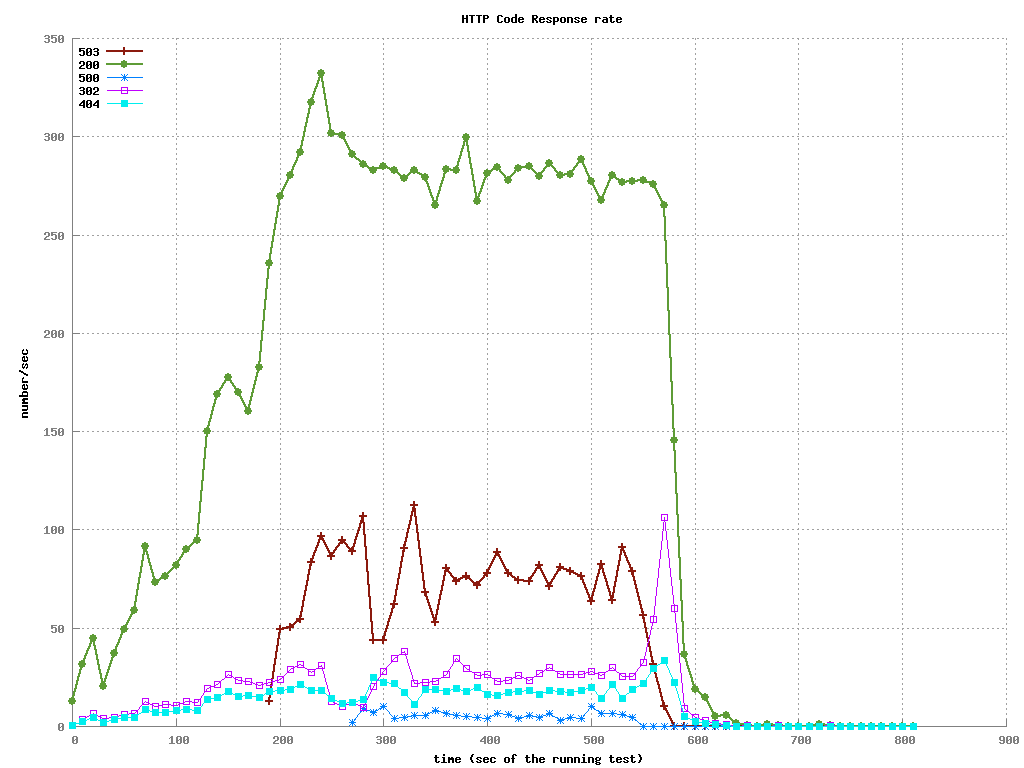
\includegraphics[width=\textwidth]{images/http_code_large.png}
        \caption{m3.large}
    \end{subfigure}
    ~ 
    \begin{subfigure}[b]{0.3\textwidth}
        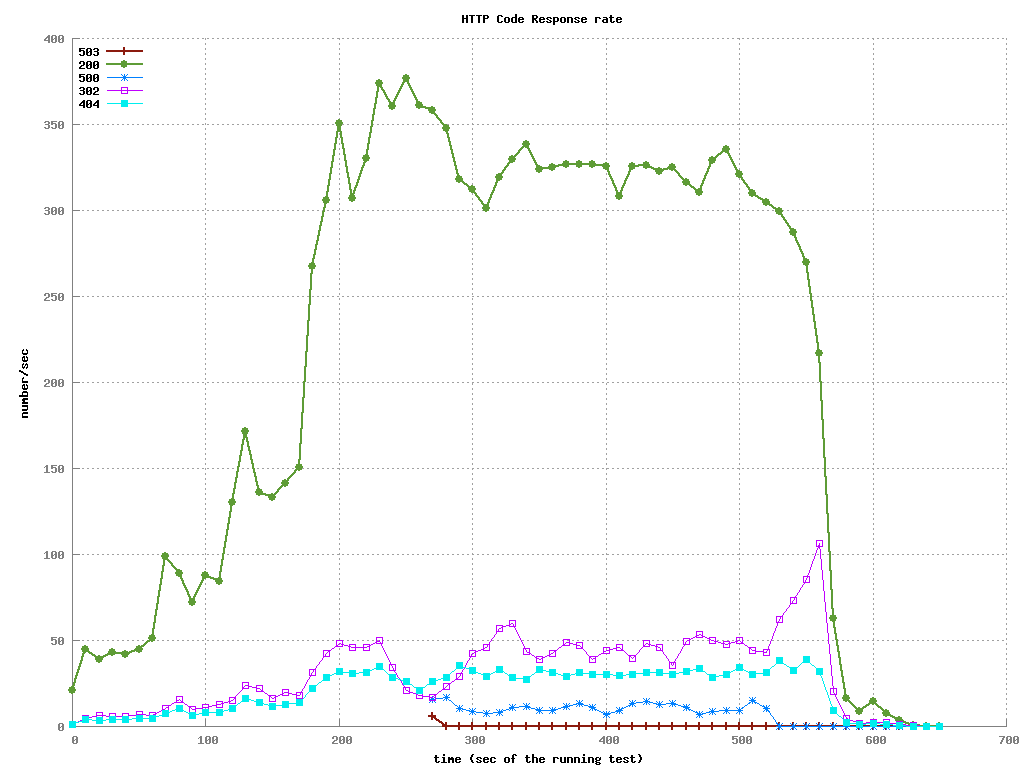
\includegraphics[width=\textwidth]{images/http_code_xlarge.png}
        \caption{m3.xlarge}
    \end{subfigure}
    \caption{HTTP code rate for three m3 instances.}
\end{figure}

\begin{figure}[h!]
    \centering
    \begin{subfigure}[b]{0.3\textwidth}
        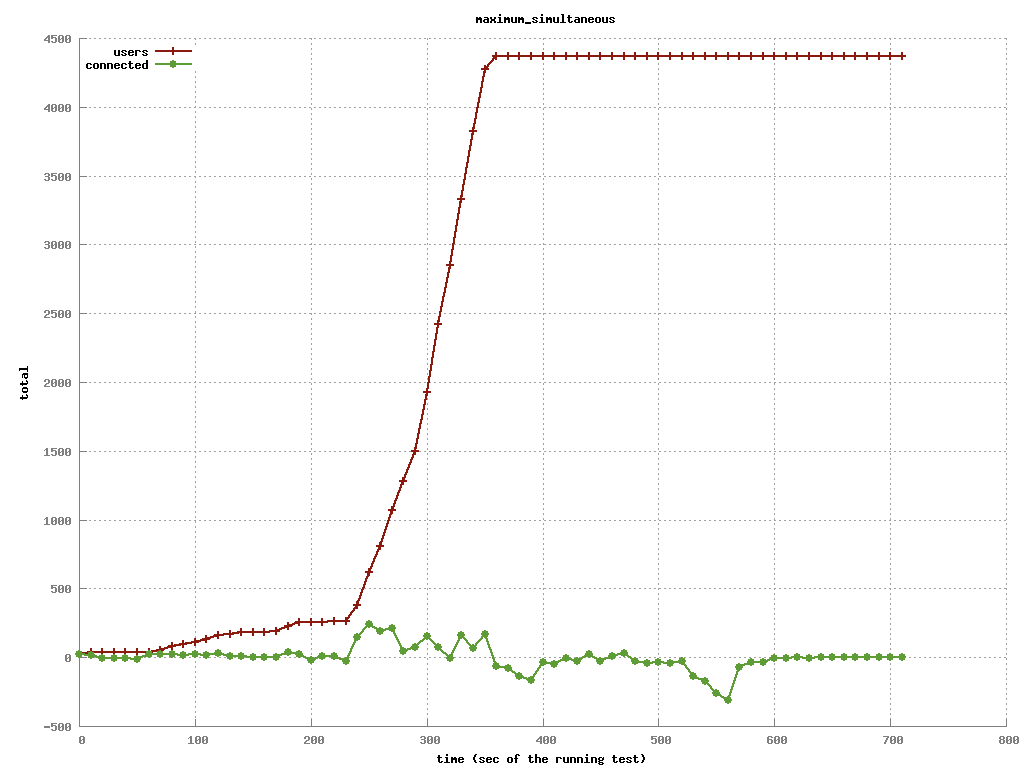
\includegraphics[width=\textwidth]{images/users_simul_medium.png}
        \caption{m3.medium}
    \end{subfigure}
    ~ 
    \begin{subfigure}[b]{0.3\textwidth}
        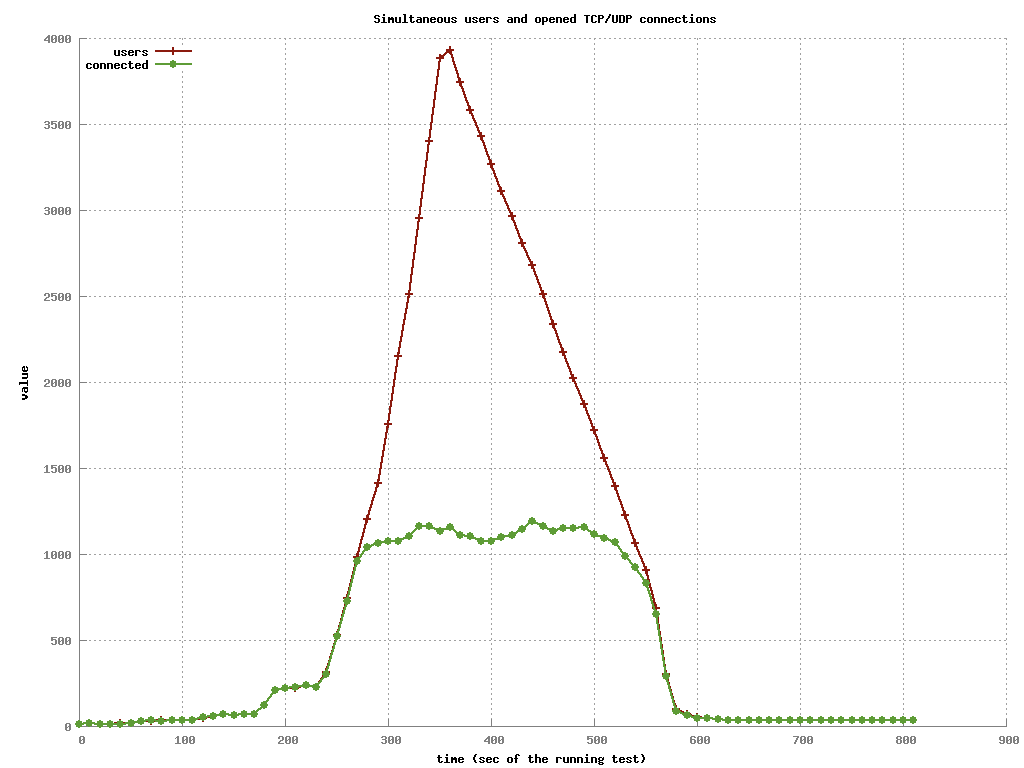
\includegraphics[width=\textwidth]{images/users_simul_large.png}
        \caption{m3.large}
    \end{subfigure}
    ~ 
    \begin{subfigure}[b]{0.3\textwidth}
        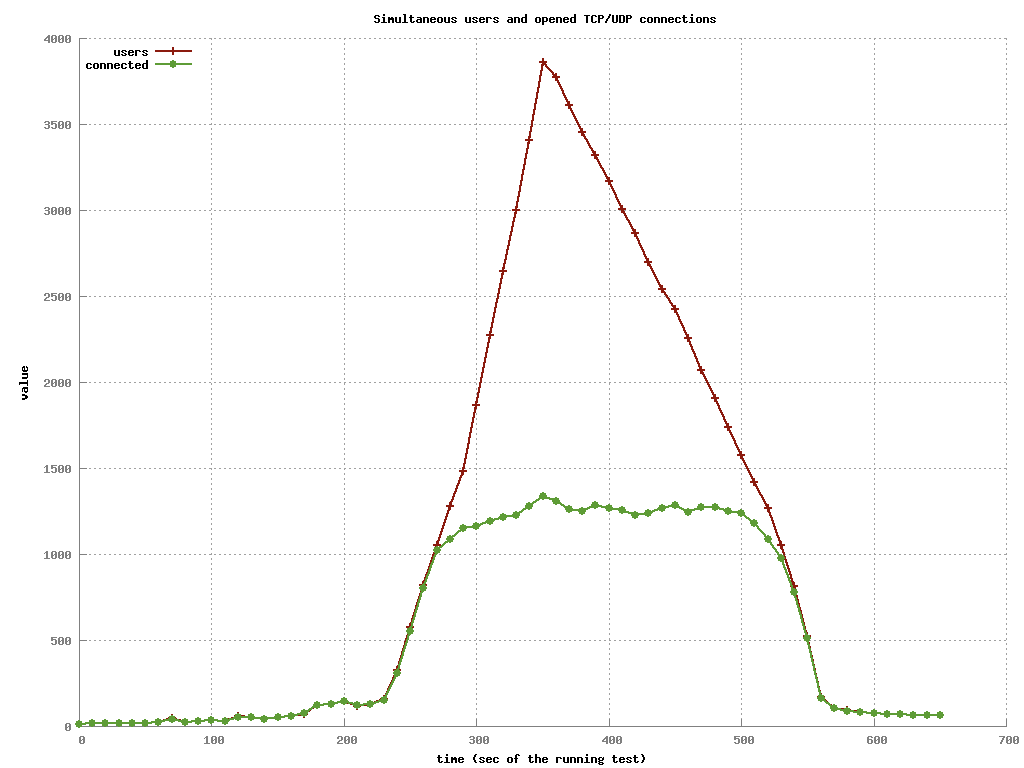
\includegraphics[width=\textwidth]{images/users_simul_xlarge.png}
        \caption{m3.xlarge}
    \end{subfigure}
    \caption{Number of simultaneous users for three m3 instances.}
\end{figure}



%\begin{figure}
%\begin{center}
%\resizebox{6in}{!}{\includegraphics*{graphimage.jpg}}
%\end{center}

%\caption{image caption}
%
%\end{figure}

\newpage
\subsection{Horizontal Scaling}

This section will discuss horizontal scaling



\end{document}